%!TEX root = ../dokumentation.tex
%%%%%%%%%%%%%%%%%%%%%%%%%%%%%%%%%%%%%%%%%%%%%%%%%%%%%%%%%%%%%%%%%%%%%%%%%%%%%%%%%%%%%%%%%%%%%%%%%%%%%%
%% Tabledefinition
\newcommand{\mc}[2]{\multicolumn{#1}{c}{#2}}
\definecolor{Gray}{gray}{0.85}
\definecolor{CamosRed}{rgb}{0.76, 0.08, 0.067}

\newcolumntype{a}{>{\columncolor{Gray}}c}
\newcolumntype{b}{>{\columncolor{white}}c}
%% End Tabledefinition
%%%%%%%%%%%%%%%%%%%%%%%%%%%%%%%%%%%%%%%%%%%%%%%%%%%%%%%%%%%%%%%%%%%%%%%%%%%%%%%%%%%%%%%%%%%%%%%%%%%%%%
\chapter{Konzeption}\label{sec:concept}
Im Folgenden wird die Konzeption der camos Crowdfunding Lösung behandelt. Hierbei wird eine Veranschaulichung des Konzepts beabsichtigt. Darüber hinaus wird die Möglichkeit einer Umsetzung mittels einer bereits etablierten Softwarelösung analysiert.

\section{Inhalte des Konzeptes}
Um eine einheitliche Definition für das Konzept zu schaffen, werden initial die einzelnen Bestandteile definiert. Grundlegend muss das Konzept alle zuvor in Kapitel \ref{sec:anforderungen_tabellarisch} aufgeführten Anforderungen erfüllen. Um den Funktionsumfang der Crowdfunding Lösung definieren zu können, wird der Prozess anhand bestehender Kriterien abgegrenzt. Durch diese Abgrenzung wird vermieden, dass das eigentliche Ziel der Lösung verfehlt wird.

\section{Abgrenzung camos Crowdfunding}
%TODO: Abgrenzung?!
Das Überarbeiten eines bestehenden Prozesses kann schnell über das Ziel hinausschießen oder es gänzlich verfehlen. Um dies zu vermeiden wird im Folgenden eine Abgrenzung der Prozessmodifikation vorgenommen.

Die camos Crowdfunding Lösung soll ein nicht-autarkes System zur Verbesserung des Ideen- und Innovationsprozesses darstellen. Das eingeführte System muss, neben den Ideen und Innovationen der eigenen Mitarbeiter, die Interessen und Belangen der Kunden berücksichtigen und somit ein Geflecht aus internem Crowdfunding und Open Innovation bilden. Ein direkter Zugang des Kunden zum System ist nicht gewünscht, weshalb eine Integration in das bestehende System notwendig ist. Unterstützend zum gegenwärtigen Prozess, sollen Ideen und Innovationen durch die Plattform anonym \emph{sichtbar} gemacht werden und den Entscheidungsgremien der Produkt- und Plattformentwicklung bereitgestellt werden.

Durch die Einführung der Crowdfunding Plattform und der einhergehenden Öffnung des Innovationsprozesses wird eine Modifikation des belohnungsbasierten Crowdfundings beabsichtigt. Die Mitarbeiter sollen durch die Bereitstellung einer virtuellen Währung eigene Ideen publizieren und gleichzeitig ihre Interessen unterstützen können. Als Stimulus soll eine zu definierende Belohnung für konstruktive Ideen eingeführt werden.

\section{Umsetzung mit Cultivate Labs Ignite}\label{sec:ignite}
Da auf dem Markt für Internes Crowdfunding bereits eine etablierte Lösung existiert, wird zunächst die Umsetzbarkeit mittels dieser analysiert. Die Software Ignite von Cultivate Labs ist eine speziell für das interne Crowdfunding entwickelte Plattform, die sich auf dem internationalen Markt bei einer Vielzahl von Kunden bewährt hat. Um die Umsetzbarkeit zu bewerten, werden die zuvor definierten Anforderungen mit dem Ignite Portfolio abgeglichen. Nach näherer Recherche hat sich herausgestellt, dass die Ignite Plattform viele Funktionen besitzt, jedoch die aus der Umfrage erhobenen Anforderungen nicht gänzlich erfüllt. Die mobile Erreichbarkeit der Plattform konnte über das Portfolio nicht gewährt werden, woraufhin eine Anfrage bei Cultivate Labs eingegangen ist, um diese Frage zu beantworten. Nach Rückantwort wurde bestätigt, dass die Mobile Erreichbarkeit derzeit nicht möglich ist und auch nicht in naher Zukunft geplant sei. Darüber hinaus sei das Zusammenfügen von Ideentickets, wie es in \ac{FA}-5 gefordert wird, nicht umsetzbar. Weitergehend ist die Auswahl von Währungen auf die Selektion von Geld begrenzt. Neutrale Währungen wie Stimmen werden nicht angeboten, was schlussendlich zum Ausschluss der Software führt. Trotz der Möglichkeit, die nicht genannten Anforderungen umzusetzen, bilden die zuvor genannten Kriterien gemeinsam einen ausschlaggebenden Grund, die Software nicht zu verwenden.

\newpage

\section{Konzeption camos Crowdfunding}\label{sec:c_crowd}
Aufgrund der nicht ausreichenden Konfigurationsmöglichkeiten seitens der Software Ignite, muss eine Lösung innerhalb der camos eigenen Programmierumgebung konzipiert werden. Die Verwendung der \ac{DSL} camos.Develop wird hierbei in Betracht gezogen, da das akquirierte Wissen innerhalb des Unternehmens dem einer \ac{GPL} überwiegt. Durch das Entwerfen einer eigenen Software wird darüber hinaus die Möglichkeit geschaffen, sie auf den eigenen Serverlandschaften des Unternehmens zu hosten, sowie jegliche Anforderungen spezifisch umzusetzen. Gleichzeitig ist die Integration in den gegenwärtigen Prozess durch die Verfügbarkeit interner Schnittstellen vereinfacht. 

Zu Beginn muss die Entscheidung für eine Plattform getroffen werden. Hierfür kommt einerseits der camos.WinClient in Frage, welcher die Entwicklung auf Desktop-Geräten unter Verwendung des Betriebssystems Windows ermöglicht. Andererseits kann auf den camos.HTML5Client zurückgegriffen werden, welcher plattformunabhängig in einem unterstützten Webbrowser läuft. Mit Hilfe der camos.Develop IDE lässt sich die Software simultan für beide Plattformen entwickeln. Es sollte hierbei jedoch der Fokus auf den camos.HTML5Client gesetzt werden, da durch \ac{FA}-3 die mobile Erreichbarkeit der Anwendung sichergestellt werden muss. Durch die native Unterstützung von Mobilgeräten im HTML5Client wird die Einhaltung der mobilen Erreichbarkeit gewahrt. Auf Grund der breiten Schnittstellenverfügbarkeit innerhalb der camos eigenen Produktlinie, kann die camos Crowdfunding Lösung direkt in den gegenwärtigen Prozess integriert werden. Hierdurch kann mittels der camos.Ticket Schnittstelle die Crowdfunding Plattform zum Intermediär des Prozesses werden. Dabei wird ermöglicht, Kundenmeinungen in den Prozess einzubinden, ohne ihnen direkten Zugriff auf die Crowdfunding Plattform zu gewähren. Dies wird arrangiert, indem Kundenanforderungen nach wie vor in camos.Ticket aufgenommen, jedoch nach ausreichender Prüfung in das Crowdfunding System übergeben werden können.

In Anbetracht der Tatsache, dass der Ideen- und Innovationsprozess nachgewiesenermaßen durch die Unsicherheit einiger Mitarbeiter beeinflusst wird, sollen Votes anonymisiert werden. Hierdurch soll diesen Mitarbeitern die Chance gegeben werden, nicht für ihre Meinung diskreditiert zu werden. Gleichermaßen geht damit die Erfüllung von \ac{FA}-10 einher. Weitergehend ist unter Beachtung von \ac{FA}-8 die Möglichkeit, Kommentare zu einzelnen Ideen erstellen zu können, einzuführen. Da diese die Meinung des Mitarbeiters vertreten, sollte das Verfassen eines Kommentars nicht anonymisiert werden. Um die Transparenz in Bezug auf den Status einer Idee gewährleisten zu können, soll mit Hilfe eines UI-Elements Plastizität geschaffen werden. Dieses Element soll die zugehörige Zahl der Unterstützer anzeigen. Damit dem Nutzer die Maximierung des Informationsflusses ermöglicht wird, soll unter Berücksichtigung von \ac{FA}-7 die Möglichkeit eingeführt werden, Ideen zu abonnieren, um somit über Änderung bzw. Akzeptanz der jeweiligen Idee informiert zu werden. 

Zur Wahrung der Übersichtlichkeit und um Ideen mit gleicher Absicht gruppieren zu können, soll eine Option zur Zusammenführung von Ideen implementiert werden. Sollte dabei der Fall auftreten, dass beide Ideen bereits Unterstützer haben, wird die Idee mit der Mehrzahl der Stimmen präferiert und im weiterführenden Verlauf als \emph{Master-Idee} gehandhabt. Ein weiterer Aspekt zur Wahrung der Übersichtlichkeit ist eine ausgiebige Filtermöglichkeit. Im Dialog mit den Stakeholdern wurde darauf hingewiesen, dass das \emph{einfache} Finden von Ideen eine große Rolle spielt, da bei einer unübersichtlichen Anzahl von Ideen der Überblick leicht verloren gehen kann. Ist es einer Idee nicht gelungen, in einem bestimmten Zeitraum ausreichend Unterstützer zu sammeln, wird dieser der Status \emph{abgelaufen} zugewiesen. 

\begin{figure}[h]
	\centering
	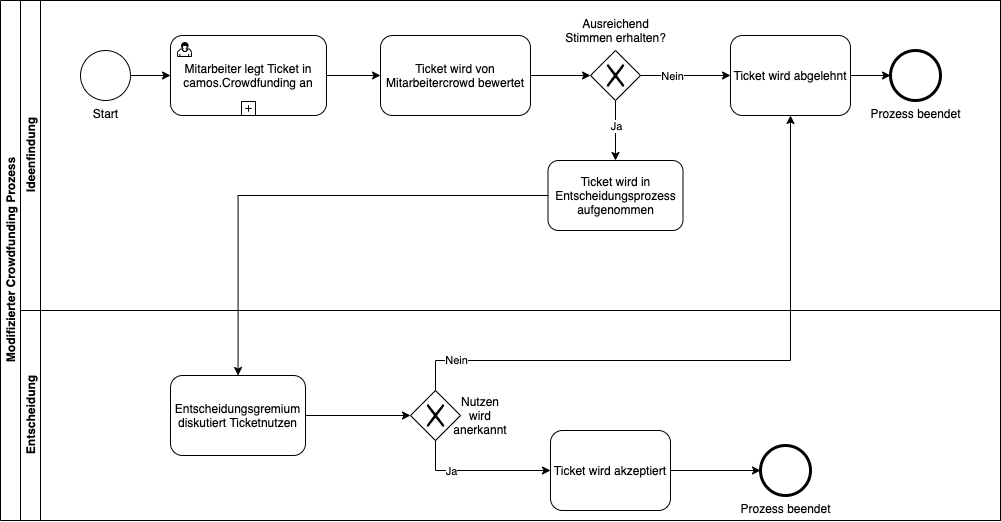
\includegraphics[width=\textwidth]{images/ProcessBPMN}
	\caption{Modifizierter Crowdfundingprozess}
	\label{fig:processbpmn}
\end{figure} 

\newpage
\subsection*{Integration in den gegenwärtigen Prozess}
Um die Plattform in ihrem zuvor beschrieben Umfang in den gegenwärtigen Prozess einbinden zu können, müssen weitergehend die in Tabelle \ref{tab:Anforderungsanalyse} aufgeführten \acs{NFA} berücksichtigt werden. Ausschlaggebend hierfür ist, die in \ac{NFA}-1 erhobene, klare Definition des Ideen- und Innovationsprozesses. Dies ist notwendig, da in Anbetracht der durchgeführten Umfrage eine Vielzahl an Mitarbeitern keine bzw. wenige Berührungspunkte mit einer unternehmensinternen Crowdfunding Lösung hatten. Um daher die Akzeptanz an eine solche Lösung zu steigern, muss die Definition des modifizierten Entscheidungsprozesses kommuniziert werden. Als Kommunikationskanal dienen die \ac{GL} und Entscheidungsgremien. Über die Definition des Prozesses hinaus, wurde von einer Vielzahl an Mitarbeitern Transparenz bezüglich der Entscheidungskriterien gewünscht. Hierbei bedarf es einer spezifischen Definition der Entscheidungskriterien, welche über einen auszuwählenden Kommunikationskanal kontinuierlich an die Mitarbeiter weitergeleitet werden. Um weitergehend Ideen und Innovationen nicht, wie im gegenwärtigen Prozess, auf Produktebene einzuschränken, sollen Mitarbeiter Ideen und Innovationen zu jeglichen Themengebieten aufstellen können. Dies fördert insbesondere passiv den Erfindergeist des einzelnen Mitarbeiters, da ihm unterbewusst die Möglichkeit der Partizipation angeboten wird. Um die Wertschätzung innerhalb des Entscheidungsprozesses nicht zu beeinträchtigen, müssen die Stimmen aller Mitarbeiter, unabhängig ihrer Position grundsätzlich gleich bewertet werden. Die Missachtung dieser Richtlinie würde sich andernfalls in einer Demoralisierung der teilnehmenden Crowd widerspiegeln, da durch ein Ungleichgewicht der Stimmwertung die Exklusivität der individuellen Stimme verloren geht. 






